%%%%%%%%%%%%%%%%%%%%%%%%%%%%%%%%%%%%%%%%%%%%%%%%%%%%%%%%%%%%%%%%%%%%%
% Richard Boardman rick@ic.ac.uk
% PhD Thesis - Department of Electrical and Electronic Engineering
% Imperial College London SW7 2BT UK
% %%%%%%%%%%%%%%%%%%%%%%%%%%%%%%%%%%%%%%%%%%%%%%%%%%%%%%%%%%%%%%%%%%%
% Improving Tool Support for Personal Information Management
% Chapter 2: Background
% Version 96, 22nd May 2004
%%%%%%%%%%%%%%%%%%%%%%%%%%%%%%%%%%%%%%%%%%%%%%%%%%%%%%%%%%%%%%%%%%%%%

%%%%%%%%%%%%%%%%%%%%%%%%%%%%%%%%
\section{Introduction}
\label{bg:intro}
%%%%%%%%%%%%%%%%%%%%%%%%%%%%%%%%

%%%%%%%%%%%%%%%%%%%%%%%%%%%%%%%%
% \section{Overview of the Chapter}
%%%%%%%%%%%%%%%%%%%%%%%%%%%%%%%
This chapter provides a conceptual grounding to the research in this thesis, and defines the key terminology used in subsequent chapters. %\footnote{This draft of ``Chapter 2 Background'' was printed \today}.

\textbf{Section~\ref{bg:pim}} provides an overview of Personal Information Management (PIM) as a fundamental aspect of computer-based activity.  \textbf{Section~\ref{bg:pim-defns}} discusses the limitations of previous definitions of PIM. Then, \textbf{Section~\ref{bg:pim-activity-cf}} outlines the view of PIM taken up in this thesis, building on the conceptual framework offered by~\citet{barreau:95}.  Lastly, \textbf{Section~\ref{bg:pim-relatedterms}} contrasts PIM with related terms such as information retrieval and information management.
% The conceptual framework builds on previous theory in the area~\cite{barreau:95}.

% provides background on software tools that support the activity of personal information management.
The second part of the chapter, \textbf{Section~\ref{bg:pim-tools}}, is concerned with the software tools that support PIM, termed \textit{PIM-tools} in this thesis. 
Firstly, \textbf{Section~\ref{bg:pimtool-defn}} defines the term PIM-tool, and describes an abstract model of a canonical PIM-tool. 
The next three sections consider the past, present, and future of PIM-tool technology.
\textbf{Section~\ref{bg:pim-history}} discusses the history of PIM-tools,  \textbf{Section~\ref{bg:current-survey}} surveys the current generation of PIM-tools, and \textbf{Section~\ref{bg:trends}} highlights a number of ongoing trends in PIM-tool design. 
Finally, \textbf{Section~\ref{bg:integration}} discusses the concept of \textit{integration between PIM-tools}, a central theme to this thesis.
% A second conceptual framework is developed in \textbf{Section~\ref{bg:pimtool-cf}} outlining a  personal information management tool
% from the first provisions of mainframe operating systems for personal storage space for users.  
% Finally \textbf{Section~\ref{bg:conclusion}} presents the chapter's conclusions and summarizes contributions towards the overall thesis.


%%%%%%%%%%%%%%%%%%%%%%%%%%%
%%%%%%%%%%%%%%%%%%%%%%%%%%%
%%%%%%%%%%%%%%%%%%%%%%%%%%%
%%%%%%%%%%%%%%%%%%%%%%%%%%%

\newpage
%%%%%%%%%%%%%%%%%%%%%%%%%%%%%%%%%%%%%%%%%%%%
\section{Personal Information Management}
\label{bg:pim}
%%%%%%%%%%%%%%%%%%%%%%%%%%%%%%%%%%%%%%%%%%%%
%% 	\item \textbf{Pervasive human activity} -- both digital and physical. 
%% define object
%% Somewhat of an overlap with the intro chapters
%% Expand on ongoing nature - use throughout the day. Small incremental changes
%% Need to talk about USER as well as TOOL and TASK

%%%%%%%%%%%%
% 2 domains
%%%%%%%%%%%%
A fundamental characteristic of human nature is to collect. In both the physical and digital domains, our personal environment (e.g. desk, wallet, computer desktop) becomes populated with the objects we accumulate as our lives unfold.

% VALUED MATERIAL
Some of these objects are acquired intentionally. We choose to keep a subset of the objects that we encounter -- those of some perceived value to us. The notion of value varies widely between the objects we keep. A brief perusal of the author's desk, the physical environment in which this thesis is being written, reveals a range of objects valued for varying reasons:  postcards kept for sentimental reasons, documents containing information required in the writing process, a cycle helmet. All these objects are valued in relation to some aspect of the author's ongoing roles and activities.
% STUFF THAT IS NOT VALUED
As well as valued material, our environments fill up with other less important objects.  This ``excess baggage'' may include objects that were once valued, but for reasons that have been long-forgotten. Other objects we do not even choose to acquire -- they just seem to appear as an implicit by-product of our lives -- for example receipts and junk mail.  Although we may wish to discard of such objects, the time and effort involved in dealing with them can be so high that we put off doing so, and they accumulate in our personal environment. % until we take the time to deal with them.
%% It may annoy us for reasons of untidiness

% Each of us makes a personal choice about how much time to devote to the management of our individual environment.
Our lives are filled with personal decisions relating to managing our possessions: what to acquire, whether and how to organize it, what to throw away, and how to go about finding things when we require them. Unless influenced by an external constraint such as a corporate clean-desk policy, this managing activity is inherently idiosyncratic.  % Two people doing the same job in the same organization are free to employ totally dissimilar management strategies.  % For example, in his study of office organization,~\citet{tm:83} noted two extremes, the \textit{messy} and the \textit{tidy}.
%% Thus it is a discretionary activity (CHECK Landauer).

Over the ages, many artefacts have been created to help people to manage the objects they collect in the physical domain.  Today, many of these are taken for granted.  For example, \citet{norman:93} discusses the invention in the late nineteenth century of the seemingly humble filing cabinet.   At the time, this device revolutionized the management of document archives.  Norman discusses the \textit{cognitive scaffolding} offered by such artefacts: they allow people to offload the overhead of organizing -- and remembering how things are organized when they need to find them -- onto the environment.
%% The humble filing cabinet is not often considered a revolutionary device in the way that Norman describes it.
%% \textit{Previous to this ...}

%% \textbf{Establish focus on digital-PIM via background in PIM-general}:
The dramatic boom in personal computing technology over the past two decades means that people now manage personal collections of \textit{digital} objects in addition to the physical objects they manage in the real-world.  Today millions of personal computer users collect and manage a wide range of digital objects such as email messages, music files, contacts, and web bookmarks.
% This digital collecting activity occurs in both home and work contexts.
%%  The term \textit{information} is used in this thesis as a general term for the various forms of digital object that people collect.
%%
%% Use of digital tools to make it easier for us
%%
%% add survey quote x% of people/households have personal computers
% Over the first quarter of 2003 an estimated 11.7 million households in the UK could access the Internet from home representing 47 per cent of all households. This is nearly twice the number three years earlier and is a continued increase from the 43 per cent reported in the first quarter of 2002.
% Retrieved from http://www.statistics.gov.uk/STATBASE/ssdataset.asp?vlnk=6935
% Expenditure and Food Survey, UK July 2003, Office National Statistics (retrieved 3 November 2003)
The term \textit{Personal Information Management}, often abbreviated to PIM, is used as an umbrella term to describe the everyday process performed by individuals as they collect, store, organize and access their collections of digital objects.  As in the physical world, a range of technologies have been developed to help people in this process, such as the folder hierarchy and search mechanisms.  This thesis aims to contribute to the HCI knowledge base to better guide the designers of such technology.
% The next section moves on to survey previous definitions of PIM from the literature.
% \textbf{Section~\ref{bg:pim-defns}} moves on to survey previous definitions of PIM. 
%% Personal Information Management (PIM) has been proposed as an umbrella term to describe the  of digital objects by an individual in their personal computing environment~\cite{lansdale:88, }. 
% In the physical world, the accumulation of information resources, typically in the form of various types of paper-based documents, is a familiar feature of our personal environments, both at work and at home.  Examples: wallet (Levy p120,~\cite{pearce:99,norman:93}). In fact physical-PIM has become driving force for much work in HCI through studies such as~\cite{tm:83}.




%%%%%%%%%%%%%%%%%%%%%%%%%%%
%%%%%%%%%%%%%%%%%%%%%%%%%%%
%%%%%%%%%%%%%%%%%%%%%%%%%%%
%%%%%%%%%%%%%%%%%%%%%%%%%%%

%%%%%%%%%%%%%%%%%%%%%%%%%%%%%%%%%%%%%%%%%%%%%%%%%%%%%%%%%%%%
\subsection{Previous Definitions}
\label{bg:pim-defns}
%%%%%%%%%%%%%%%%%%%%%%%%%%%%%%%%%%%%%%%%%%%%%%%%%%%%%%%%%%%%
%% Word: imprecise definition
%% The term personal information management has not been tightly defined in the literature.
%% Think about Barreau's framework as a basic task decomposition, although one that is ONGOING
% In this section previous definitions of personal information management are surveyed. These definitions focus on personal information management as an everyday activity carried out by computer users.
%% \textit{Is copying and pasting a paragraph of text between documents personal information management?}
%% ADD: why is a definition important?
%%%%%%%%%%%%%%%%%%%%%%
% SIMPLE definition
%%%%%%%%%%%%%%%%%%%%%%
% PIM is information management as performed by an individual user for their own needs. 
% PIM can be defined very simply as \textit{information management performed by an individual for their own needs}.  However, such a high-level definition does not define what the information is being managed, and what constitutes ``management''.

%%%%%%%%%%%%%%%%%%%%%%%%%%%%%%%%%%%%%%%
% Lack of consensus on a definition
%%%%%%%%%%%%%%%%%%%%%%%%%%%%%%%%%%%%%%%
% Terms used in different ways, e.g. ``archiving''
\citet{Whittaker-rta:00} observe the lack of systematic research within Human-Computer Interaction (HCI) on many everyday computing activities including PIM.  One problem they identify is the lack of consensus regarding the definition of key terms.  This means that researchers doing new work in the area add new definitions to the wide range of candidates already available.  This section surveys some previous definitions of PIM and argues the need for a more systematic definition.

%%%%%%%%%%%%%%%%%%%%%%%%%%%%
% PIM = store to retrieve?
%%%%%%%%%%%%%%%%%%%%%%%%%%%%
Many definitions of PIM draw from a traditional information management perspective -- that information is stored so that it can be retrieved at a later date.  For example,~\citet{Bellotti:02a} describe PIM as: \textit{``the ordering of information through categorization, placement, or embellishment in a manner that makes it easier to retrieve when it is needed''}.  Such definitions are founded on the assumption that information is stored to facilitate later retrieval.
%%  It may also involve a great deal of information related to coordination and collaboration (collaborative information management). It may involve resources such as piles, collections, file hierarchies, notes, to-do lists, calendars, contact managers and so on."'}.
% Thus there is more to personal information management than is reflected in the above definitions.
%% recall/recognition and classification


%%%%%%%%%%%%%%%%%%%%%%%%%%%%
% What about reminding?
%%%%%%%%%%%%%%%%%%%%%%%%%%%%
% %% We need to look beyond the traditional information management perspective that focuses on storing items for future retrieval.
% (i.e. to contextualize their work activity).
Similarly, \citet{ml:88} defines PIM as \textit{``the methods and procedures by which we handle, categorize, and retrieve information on a day-to-day basis''}.  However, Lansdale notes that enabling retrieval is only one reason for managing information, referring to the work of \citet{tm:83} who observed the \textit{reminding} affordance of paper documents.  Malone describes how people do not only manage documents to find them again, they also do so to remind themselves of tasks to perform.  Although Lansdale acknowledges the various ways in which information can be used, his definition can be criticized for not defining what is meant by ``handling''.

%%%%%%%%%%%%%
% BARREAU
%%%%%%%%%%%%
% She conceptualizes a PIM system as \textit{``an information system developed by, or created for, an individual in a work environment''}.  
\citet{barreau:95} conceptualizes  a PIM system as \textit{``an information system developed by, or created for, an individual in a work environment''}.  She considers how a PIM system enables the construction of a collection of items, which constitute a personal information space. Barreau describes five functions provided by a PIM system:
% Barreau's definition highlights the fact that personal information management is a high-level activity, one that consists of multiple sub-activities.

\begin{enumerate}

%%%%%%%%%%%%%%%%%
% ACQUISITION
%%%%%%%%%%%%%%%%
%% Barreau: the methods and rules by which information is added to the system.
% (e.g. the creation of information by the user, or the downloading of information from the internet).
\item The \textit{acquisition} of items into the PIM system, including the definition, grouping, and naming of new information (e.g. the saving of newly created or downloaded information).

%%%%%%%%%
% ORG
%%%%%%%%%
\item The \textit{organization} of items within the system (e.g. filing items into folders). 
%% Barreau notes the different classifying rules used based up on the level of granularity of the workload being supported

%%%%%%%%%%%%%%
% MAINTENANCE
%%%%%%%%%%%%%%
% (e.g. deleting items, backing up items, archiving items, and updating items). 
% Barreau: dictated by circumstance
% Barreau: update, delete, archive, backup
\item The \textit{maintenance} of the system in terms of updating, archiving and deleting items\footnote{Another source of terminological confusion in the area is the lack of definition for terms such as \textit{archiving}. Some researchers use archiving to refer to the filing of an item within a folder, e.g.~\citep{Whittaker-email:96}.  In this thesis, Barreau's interpretation of archiving is employed: the removal of an item from a collection for storage elsewhere.}.

%%%%%%%%%%%%%%
% RETRIEVAL
%%%%%%%%%%%%%%
\item The \textit{retrieval} of items via search or browsing, as driven by the user's information needs.
% Common retrieval mechanisms include the browsing of items arranged in semantic categories (e.g. folders) or spatially on the desktop, sorting items in order of metadata, or content/keyword-based searching.

\item The \textit{presentation} of retrieved information in an appropriate output format. % (\textit{``the procedures for producing the various outputs desired''})

\end{enumerate}

%%%%%%%%%%%%%%%%%%%%%%%%%%%%%%%
% TOWARDS A NEW DEFINTION
%%%%%%%%%%%%%%%%%%%%%%%%%%%%%%%
%Another limitation of previous definitions is that they do not specify what constitutes information, and what is special about personal information.
%However these definitions do not define personal information or what constitutes management.  Barreau comes the closest but has several limitations as follows:
%\begin{enumerate}
%\item She limits to work
%\item She includes ``editing'' -- surely then this involves everything performed on a computer
%\end{enumerate}
%\textbf{Section~\ref{bg:pim-activity-cf}} builds on these previous definitions by building up a conceptual framework relating to personal information management.
Although Barreau's definition conveys the multi-faceted nature of ``handling'' items, it can be criticized on several counts.  Primarily, she includes the \textit{updating} of items in her definition of the maintenance aspect of PIM.  In contrast, the author takes the view that updating items (e.g. editing a file or a diagram) is not part of PIM.
% In particular, PIM is explicitly distinguished from the modification of information. 
Rather than proposing a brand new definition, the next section modifies Barreau's framework to deal with this and a number of other limitations.  This new definition represents the view of PIM taken up in this thesis. %, and is later used to define the term PIM-tool.

% Firstly, definitions of \textit{information} and \textit{personal information} are offered.  It is argued that ``personal information'' in particular is an ambiguous term that requires careful specification.





%%%%%%%%%%%%%%%%%%%%%%%%%%%%%%%%%%%%%%%%%%%%%%%%%%%%%%%%%%%%%%%%%%%%%%%%%%
\subsection{Defining Personal Information Management Step by Step}
\label{bg:pim-activity-cf}
%%%%%%%%%%%%%%%%%%%%%%%%%%%%%%%%%%%%%%%%%%%%%%%%%%%%%%%%%%%%%%%%%%%%%%%%%%
%%
%%The following criticisms can be levelled at definitions to date:
%%\begin{enumerate}
%%	\item All three of these definitions is the assumption that the fundamental reason for managing information is to facilitate its retrieval at a later date.
%% \end{enumerate}

This section builds up a step-by-step definition of PIM in three stages:
%% The definition consists of the following three stages:
\begin{enumerate}

\item Firstly, a definition of \textit{information} is presented.
\item This is specialized to form a definition of \textit{personal information}.
\item The final step is to define the term \textit{PIM}.  This definition in turn used to define the functionality provided by a PIM-tool in \textbf{Section~\ref{bg:pim-tools}}.
\end{enumerate}

% The definition of personal information management is used in turn to define what it means for a software tool to support \textit{personal information management}, and to scope out the work carried out in the thesis.


%%%%%%%%%%%%%%%%%%%%%%%%%%%%%%%%%%%%%%%%%%%%%%%
\subsubsection{Defining ``Information''}
%%%%%%%%%%%%%%%%%%%%%%%%%%%%%%%%%%%%%%%%%%%%%%%
%% This is a very general definition and includes 
%% Need to cite definition of ``information''
%% bits/also known as content?
%% http://pespmc1.vub.ac.be/ASC/INFORMATION.html
%% that which reduces uncertainty. (Claude Shannon);
%% 2) that which changes us. (Gregory Bateson), Information is the meaning
% of the representation of a fact (or of a message) for the receiver.
%% Document -- Buckland
%% Bits -- Raskin
%% Angela -- data/information
%% Jens -- why not box in Excel?
%% Losee - Information may be defined as the characteristics of the output of a process, these being informative about the process and the input.  - http://www.ils.unc.edu/~losee/b5/book5.html
%% NB: this is personal information!! Are we jumping ahead?
%%%%%%%%%%%%%%%%%%%%%%%%%%%%%%%%%%%%%%%%%%%%%%%%%%
% http://www.aslib.co.uk/info/glossary.html
% Information: an assembly of data in a comprehensive form capable of communication and use 
% Knowledge: information evaluated and organised in the human mind so that it can be used purposefully
%%%%%%%%%%%%%%%%%%%%%%%%%%%%%%%%%%%%%%%%%%%%%%%%%%

% \textit{Information} is defined as any set of bits with carries meaning for an individual, such as text or a graphic image.
\textit{Information} has been defined as \textit{``an assembly of data in a comprehensive form capable of communication and use''}~\citep{IEILS:03}.  Here, information is defined more loosely as any assembly of data which carries some meaning for one or more people. % Indeed, it may not necessarily be useful or communicable. 
% What is crucial, is that it means something to one or more people.
This thesis focuses on information in the digital domain: arrangements of bits which carry meaning for one or more people, for example a paragraph of text or an image.  Henceforth, the term information is used to designate information in a digital context.  The next stage is to distinguish \textit{personal information} from information in general.




%%%%%%%%%%%%%%%%%%%%%%%%%%%%%%%%%%%%%%%%%%%%%%%
\subsubsection{Defining ``Personal Information''}
%%%%%%%%%%%%%%%%%%%%%%%%%%%%%%%%%%%%%%%%%%%%%%%
%%%%%%%%%%%%%%%%%%%%%%%%%%%%%%%%%%%%%%%%%%%%%%%
% \subsubsection{Alternatives interpretations of ``Personal Information''}
%%%%%%%%%%%%%%%%%%%%%%%%%%%%%%%%%%%%%%%%%%%%%%%
%%%%%%%%%%%%%%%%%%%%%%%%%%%%%%%%%%%%%%%%%%%%%%%%%%%%%%%
%% Add contrast with private information (see above)
%%%%%%%%%%%%%%%%%%%%%%%%%%%%%%%%%%%%%%%%%%%%%%%%%%%%%%%
%% Consider created/downloaded by user
%%%%%%%%%%%%%%%%%%%%%%%%%%%%%%%%%%%%%%%%%%%%%%%%%%%%%%%%%%%%%%%%%%
%% Need to define static/dynamic/executable/binary information
%%%%%%%%%%%%%%%%%%%%%%%%%%%%%%%%%%%%%%%%%%%%%%%%%%%%%%%%%%%%%%%%%%
\textit{Personal information} is an ambiguous term with a number of possible interpretations.
\begin{enumerate}

\item One interpretation is \textit{information about an individual} (i.e. where that individual is the subject matter of the information).  One common context for this usage is to describe the information stored by an institution about an individual  (e.g. date of birth, credit card number).  In this case, the information is not directly managed by the individual concerned.

\item A second interpretation is \textit{the information managed and stored within personal organizer software} ~\citep{web-rosenberg:99}.  In this sense digital personal information includes appointments, contacts, and to-do items -- but not information stored outside that specific tool, such as files stored in the file system. 
%%
%% Check Chandler

\end{enumerate}

%%%%%%%%%%%%%%
% DEFINITION
%%%%%%%%%%%%%%
% Notice that the definition of personal information used in the thesis is independent of technological format subsumes personal information stored in a personal organizer.	
% differentiates between personal information and private information. Personal information is that which is \textit{owned} by an individual, such as their files, diaries and books.  Private information is considered confidential by an individual, but is not necessarily owned by them.
% Note that Lansdale's definition does not specify what the subject matter of the information is -- what is crucial is that it is owned and actively managed by the individual.
% The individual is the subject of the information, but does not own the information: instead it is controlled and \textit{managed} by the . A common example is personal information recorded during the process of making a financial transaction on-line. Releasing such details to outside interests carries significant privacy implications and is the focus on significant development focus~\cite{p3p:03}.
%%%%%%%%%%%%%%%%%%%%%%%%%%%%%%%%%%%%%%%%%%%%%%%%%%%%%%%%%%%%
% NB: may not own in the legal sense
In the context of this thesis, personal information is defined as \textit{information owned by an individual, and under their direct control}.  In other words, the owning individual is able to alter or delete the information without going through an intermediary.  Note that this definition is independent of (1) the subject matter of the information, (2) the software application in which it is managed, and (3) the digital device on which it is stored.
%%%%%%%%%%%%%%%%%%%%%%
% UNITS OF ANALYSIS
%%%%%%%%%%%%%%%%%%%%%%
The units of analysis in this thesis are those of \textit{items} and \textit{collections} of personal information:
\begin{itemize}
%%%%%%%%%%%
% ITEM
%%%%%%%%%%%
% An \textit{item of information} is a self-contained unit of information (i.e. one that can exist in an independent form on a computer).
% In a personal computer, items of information are stored in a particular technological format such as file, email, bookmark, contact, calendar appointment and to-do item.  
% The term item is used to describe self-contained units of digital personal information such as 
\item An \textit{item} is a self-contained unit of information. In the digital domain, items of personal information exist in a range of \textit{technological formats} such as files, email, bookmarks, contacts, to-do item, and so on.  Note that in this thesis, a sentence or paragraph is not considered to be a unit of personal information, but rather a sub-unit.  Items may possess \textit{metadata attributes}, further information describing the content of the item.  Attributes may be system-defined (e.g. file size) or user-defined (e.g. title).  % Items may be classified within a semantic category (e.g. filed within the ``Chicago'' folder) or within a spatial category (e.g. placed in the top-left corner of the desktop).
%% Items contain \textit{information content} (the meaningful bits). 

%%%%%%%%%%%%%%%%%%%%%%%%%%%%%%%%%%%%
% A collection of information
%%%%%%%%%%%%%%%%%%%%%%%%%%%%%%%%%%%%
% A \textit{collection} of items of information is a stand-alone/self-contained set of items. 
\item A \textit{collection} of personal information is a self-contained set of items. Typically the members of a collection share a particular technological format and are accessed through a particular application\footnote{The main exception is the file system which can contain items (files) in a range of technological formats, e.g. spreadsheets, images and text documents.}.  Each collection can be considered as a \textit{personal information space} that is constructed by the user~\citep{da:98}. Example collections of personal information include electronic messages, managed with an email tool, and the set of contacts within an address book.

\end{itemize}
% In the context of a typical desktop computer, personal information includes all information stored in all applications, including personal organizers, files in the file system, contacts, calendar entries, email messages and so on.

% LINK FORWARD
% Note that digital personal information can exist on a range of devices -- for example computers, mobile phones and PDA devices. See next section.
% Based on this understanding of personal information, \textit{PIM} can now be defined.



%%%%%%%%%%%%%%%%%%%%%%%%%%%%%%%%%%%%%%%%%%%%%%%%%%%%%%%%%
\subsubsection{Defining ``Personal Information Management''}
%%%%%%%%%%%%%%%%%%%%%%%%%%%%%%%%%%%%%%%%%%%%%%%%%%%%%%%%%%
% \textbf{Classic HCI analysis}: the user, the tool, the task, context
%	\item Who is the user? -- everyone!
%	\item What is the tool? -- PIM tools
%	\item What is the activity? -- a long story!
%	\item And what about context of this activity?
% THINK: need to define each sub-activity in turn?
% Acquisition -a dding item to a collection and assigning metadata (explicit plus implicit)
%%%%%%%%%%%%%%%%%%%%%%%%%%
% DICTIONARY DEFINITION
%%%%%%%%%%%%%%%%%%%%%%%%%%
The Oxford English Dictionary defines ``management'' as \textit{``the process of dealing with or controlling things (noun), to be in charge of an undertaking, to administer, to regulate (verb)''}. 
%% amusingly also means to succeed (just) in achieving something difficult
%%%%%%%%%%%%%%%%%%%%%%
% PIM Definition
%%%%%%%%%%%%%%%%%%%%%%
%is here defined as the activity performed by an individual in
%the process an individual carried out in dealing with and controlling their collections of personal information.
Therefore, based on the above definition of personal information, PIM can be defined as \textit{the management of personal information as performed by the owning individual}.
% Furthermore that management activity is carried out for the individual's own needs.
%% an activity, carried out by an individual, of \textit{managing}, looking after, handling, their collections of personal information, their files, email and contacts. Thus the example is the management of an information by an individual for their own use.
%% The key is who is doing the management of the information by an individual for their own use. 
%% \textit{Construction of an information space. Customization of general-purpose workspace. Beyond storage and retrieval}
The conceptual framework offered by~\citet{barreau:95} is adopted in this thesis to denote the sub-activities that constitute ``management''.  However, a number of changes are made to Barreau's conceptualization as follows:
%		\item acquisition -- Archive as safekeeping (Levy).
%		\item storage/organization -- structure to handle complexity. Levy: anxiety of order, tidying
%		\item maintenance
%		\item retrieval.
% In this thesis, the following changes are applied to the framework:
\begin{enumerate}

%%%%%%%%%%%%%
% UPDATING
%%%%%%%%%%%%%
\item As noted above, Barreau included the \textit{updating} of information in her definition of the maintenance sub-activity.  Here the modification of items (e.g. editing of files) is considered outside the scope of PIM. Once an item of information is retrieved from a collection, it may be edited and re-saved (effectively re-acquired).  However what happens between the retrieval and re-saving is not considered part of PIM.
	
%%%%%%%%%%%%%%%%%%%%
% WORK OR LEISURE
%%%%%%%%%%%%%%%%%%%%
\item Barreau defines PIM as being carried out in a work context. Here it is defined as the managing of personal information in any context -- work or leisure.

%%%%%%%%%%%%%%%%%%%%%%%%%%%%%
%% FOUR PIM SUB-ACTIVITIES
%%%%%%%%%%%%%%%%%%%%%%%%%%%%%
%% Acquisition can be implicit or explicit. Two fundamental types: downloading, creation. Resaving
%%
%% Organization can also be implicit or explicit.
%% 
%% Finally retrieval can also be implicit or explicit -- search and browse.
%% 
%% \textbf{Different strategies for each sub-activity}  along with different motivations?
%% \textbf{Very complex/multifaceted activity} -- see section on nature of PIM below. e.g. ongoing, an activity in the large
%% 	\item Task granularity -- cue supporting/production discussion. NB even these sub-processes are complex!
\item Barreau defined PIM in terms of the functions provided by a PIM-system: \textit{acquisition}, \textit{organization}, \textit{maintenance}, \textit{retrieval} and \textit{output}.  In this thesis, PIM is conceptualized as a user activity.  
% \item Acquisition, organization, maintenance and retrieval of information can be \textit{explicit} (performed intentionally by the user) 
% In other words the other ``contextualizing'' functions such as reminding identified by~\cite{tm:83} are encompassed in the definition.
The first four of Barreau's functions equate to PIM sub-activities performed by a user: the \textit{acquisition} of items to form a collection of personal information, the \textit{organization} of items, the \textit{maintenance} of the collection, and the subsequent \textit{retrieval} of items. Barreau also highlights \textit{output} as a key PIM-system function.  Since this is performed automatically by the computer in current PIM tools, it is not included as a sub-activity.  Furthermore, reminding is not considered to be a PIM sub-activity.  Instead, the view is taken that items may be acquired and arranged (as part of PIM) to enable reminding.  \textbf{Figure~\ref{fig:chapter1_pim_model}} illustrates the view of PIM taken in this thesis.  

%Information is not only acquired and stored with the intent of retrieving it at a later date. As noted by Lansdale and Malone, an item information within a collection may simply act as a reminder. Indeed, information may not be retrieved at all.

\end{enumerate}



% %%%%%%%%%%%%%%%%%%%%%%%%%%%%%
% FIGURE - CONCEPTUALIZATION OF PIM
% %%%%%%%%%%%%%%%%%%%%%%%%%%%%%
\begin{figure}[hbtp]
	\begin{center}
		\leavevmode
		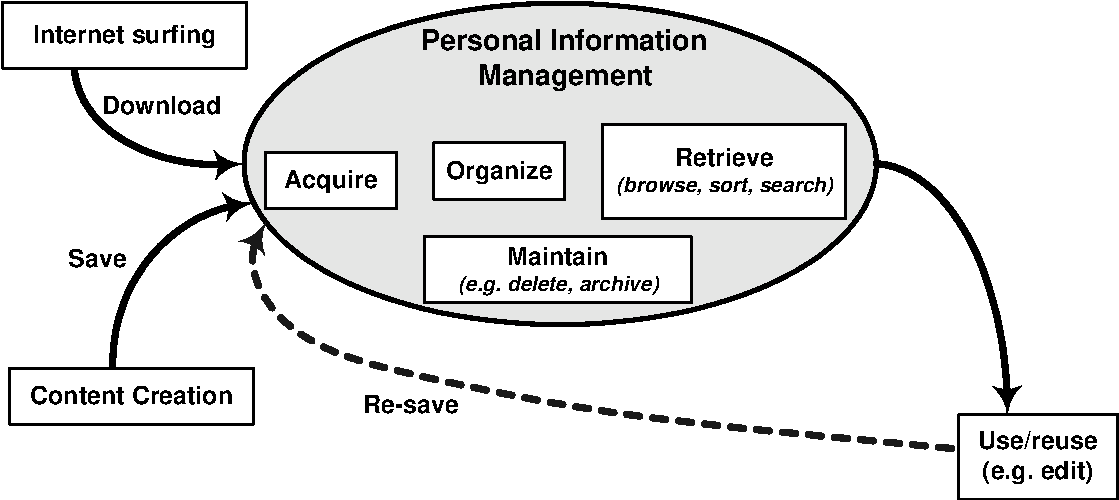
\includegraphics[height=4cm]{pictures/bg/BG-PimModel.pdf}
		\caption{Four PIM sub-activities: acquisition, organization, maintenance and retrieval}
		\label{fig:chapter1_pim_model}
	\end{center}
\end{figure}


%% Towards a distributed view
%% Cross-tool
%% Set of parallel/inter-related PIM systems
Barreau treats the computer as one monolithic PIM system, centred on the file system.  This thesis builds up the case that the computer is best conceptualized as a set of PIM systems, each denoted by the software application that allows a user to manage a collection of personal information in a particular technological format. Examples include the email collection, the bookmark collection, and the file collection.  For now this framework is offered as a description of the activities performed by an individual in each collection of personal information.
% This theme -- that the computer is best conceptualized as a set of parallel PIM systems -- is developed over the course of the thesis.




%%%%%%%%%%%%%%%%%%%%%%%%%%%%%%%%%%%%%%%%%%%%
\subsection{Comparison between PIM and Related Terms}
\label{bg:pim-relatedterms}
%%%%%%%%%%%%%%%%%%%%%%%%%%%%%%%%%%%%%%%%%%%%%%
 % Firstly, the term PIM is compared with related terms.
%c This section differentiates PIM from similar terms such as \textit{information management}, \textit{knowledge management}, and \textit{information retrieval}.

%% Relate to other "`applied"' areas \textit{(NB: generally these have been much more researched -- indeed IR has its own conferences)}:


%%%%%%%%%%%%%%%%%%%%%%%%%%%%%%%%%%%%%%%%%%%%%%%%%%%%%%%%%%%%%%%%%%%%%%%%
\subsubsection{Information Management}
%%%%%%%%%%%%%%%%%%%%%%%%%%%%%%%%%%%%%%%%%%%%%%%%%%%%%%%%%%%%%%%%%%%%%%%%
% http://www.aslib.co.uk/info/glossary.html
% Information: an assembly of data in a comprehensive form capable of communication and use 
% 
% Knowledge: information evaluated and organised in the human mind so that it can be used purposefully
% Information Management (IM): an imprecise term covering the various stages of information processing from production to storage and retrieval to dissemination towards the better working of an organisation; information can be from internal and external sources and in any format
% Knowledge Management (KM): again an imprecise term very similar to information management the main difference is the sharing (mapping) of information and experience of many individuals towards the betterment of an organisation, rather than information remaining with different individuals working separately towards the same goal
% The key difference between PIM and IM/KM is the entity which is carrying out the managing activity. 
\textit{Information Management} (IM) has been described as \textit{``the application of management principles to the acquisition, organization, control, dissemination and use of information relevant to the effective operation of organizations of all kinds''}~\citep{wilson:02a}.  In other words, the term IM typically relates to an organizational context\footnote{The term \textit{knowledge management} (KM) is sometimes used in a similar sense, somewhat controversially, to refer to IM as performed by a large institution such as a company~\citep{wilson:02b}.}. In contrast, with PIM, the scope of interest is limited to that of an individual user. % Indeed the PIM activities of all an organizations members can be seen to contribute to the overral 
%%  WILSON: Information here refers to all types of information of value, whether having their origin inside or outside the organization, including data resources, such as production data; records and files related, for example, to the personnel function; market research data; and competitive intelligence from a wide range of sources. Information management deals with the value, quality, ownership, use and security of information in the context of organizational performance}

%%%%%%%%%%%%%%%%%%%%%%%%%%%%%%%%%%%%%%%%%%%%%%%%%%%%%%%%%%%%%%%%%%%%%%%%
\subsubsection{General Information Management}
%%%%%%%%%%%%%%%%%%%%%%%%%%%%%%%%%%%%%%%%%%%%%%%%%%%%%%%%%%%%%%%%%%%%%%%%
\citet{Bergman:03} compare PIM with what they term \textit{General Information Management} in which a professional -- such as a librarian - manages information for other people.  PIM is differentiated by its focus on an individual managing information \textit{for his or her own use}.  Managing information for other users is outside the research scope of this thesis.
% An analogy in the physical world, would be that of a personal book collection compared with a library. 
%% information storage and retrieval
%% digital libraries (GIS)

%%%%%%%%%%%%%%%%%%%%%%%%%%%%%%%%%%%%%%%%%%%%%%%%%%%%%%
\subsubsection{Collaborative Information Management}
%%%%%%%%%%%%%%%%%%%%%%%%%%%%%%%%%%%%%%%%%%%%%%%%%%%%%%
%% \textit{Although may be side-effects through shared drives etc.  Contrast with shared systems where managing done by someone else~\cite{blomberg:96}. Of course there is an overlap but here, for the purpose of this thesis we ignore shared systems. Compare with shared systems. Discuss as difference between public library and personal collection. Some overlap with shared systems (e.g. shared group drives, but here focus on individual -- a pragmatic assumption)}
Another type of IM is \textit{Collaborative Information Management} (CIM) when a collection of information is managed by multiple users. For example, a team may share information via a communally managed network drive.  CIM raises numerous issues such as the need for a shared vocabulary for naming and categorizing items~\citep{berlin:93}.  This thesis focuses on PIM performed by an individual for their own dedicated use. Issues relating to CIM are outside the scope of this research\footnote{Note that a particular collection of information (e.g. a network drive) may be used for both PIM and CIM.  For instance, it is possible that team members may store personal information, not intended for others, on one area of a shared network drive.}.  

%%%%%%%%%%%%%%%%%%%%%%%%%%%%%%%%%%%%%%%%%
\subsubsection{Information Retrieval}
%%%%%%%%%%%%%%%%%%%%%%%%%%%%%%%%%%%%%%%%%

Information Retrieval (IR) has been defined as \textit{``the study of systems for indexing, searching, and recalling data, particularly text or other unstructured forms''}~\citep{Weiss:97}. IR is a discipline in its own right, served by a range of journals and conferences. %, as well as SIGIR, an ACM special interest group.

Here it is argued that PIM can be considered a high-level activity which involves IR in two of its sub-activities: \textit{acquisition} and \textit{retrieval}. \textbf{Figure~\ref{fig:chapter2_pim_and_ir}} illustrates the relationship between PIM and IR.  Firstly, the acquisition of an item may involve the retrieval of the item from a remote information system such as a website.  Secondly, the PIM sub-activity of retrieval is equivalent to IR within the context of an individual's personal collection. % The first case, the act of retrieving information from a remote information source is not considered part of PIM, whilst the second case, retrieving information form a personal collection, is.
%%  \textit{THINK: PIM long-term, IR short-term}
%% information foraging, information-seeking , knowledge acquisition

% %%%%%%%%%%%%%%%%%%%%%%%%%%%%%%%%%%%%%%%%%%%%%%%%%%%%%%%%%%%%%%%
% FIGURE - The Relationship between PIM and information-retrieval
%%%%%%%%%%%%%%%%%%%%%%%%%%%%%%%%%%%%%%%%%%%%%%%%%%%%%%%%%%%%%%%%%
\begin{figure}[hbtp]
	\begin{center}
		\leavevmode
		%% [height=2in, width=.9 \textwidth]
		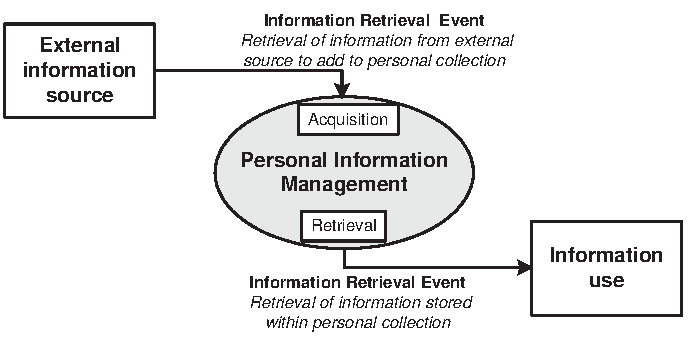
\includegraphics[height=4cm]{pictures/bg/BG-RshipPIMandIR.pdf}
	\end{center}
	\caption{The relationship between PIM and Information Retrieval}
	\label{fig:chapter2_pim_and_ir} 
\end{figure}

% LINK to \textbf{Section~\ref{bg:pim-tools}} 
% The next section moves on to consider the software tools which allow computer users to manage collections of personal information.

%%%%%%%%%%%%%%%%%%%%%%%%%%%
%%%%%%%%%%%%%%%%%%%%%%%%%%%
%%%%%%%%%%%%%%%%%%%%%%%%%%%
%%%%%%%%%%%%%%%%%%%%%%%%%%%

\newpage
%%%%%%%%%%%%%%%%%%%%%%%%%%%%%%%%%%%%%%%%%%%%%%%%%%%%%%%
\section{Personal Information Management Tools}
\label{bg:pim-tools}
%%%%%%%%%%%%%%%%%%%%%%%%%%%%%%%%%%%%%%%%%%%%%%%%%%%%%
%%%%%%%%%%%%%%%%%%%%%%%%%%%%%%%%%%%%%%%%%%%%%%%%%%%%%%
%% Consider PIM tools in terms of artifact theory
%%%%%%%%%%%%%%%%%%%%%%%%%%%%%%%%%%%%%%%%%%%%%%%%%%%%%%
%% Complex artifacts to reflect nature of PIM.  Myriad features and claims in Carroll's language. Think about the implicit theories that they manifest, although not explicitly expressed in these terms can be interpreted
%%%%%%%%%%%%%%%%%%%%%%%%%%%%%%%%%%%%%%%%%%%%%%%%%%%%%%
%% Dix: artefacts embody theories (Carroll), experiences, assumptions
%%%%%%%%%%%%%%%%%%%%%%%%%%%%%%%%%%%%%%%%%%%%%%%%%%%%%%
%% Can we consider as part of HCI knowledge
%%%%%%%%%%%%%%%%%%%%%%%%%%%%%%%%%%%%%%%%%%%%%%%%%%%%%%
%% Consider as environments rather than tools
%%%%%%%%%%%%%%%%%%%%%%%%%%%%%%%%%%%%%%%%%%%%%%%%%%%%%%

% IMPLICIT/EXPLICIT
% However they may also be performed automatically by the system. 
% Indeed, the four above sub-activities may also be \textit{implicit}, performed automatically by the system. Examples are provided in the context of the organizing sub-activity. An example of explicit organization would be the manual placement of a file within a folder. An example of implicit organization would be the default alphabetical ordering of items based on metadata that has been automatically assigned.  

% \textbf{Section~\ref{bg:pim}} discussed personal information management as an activity performed by individual computer users. This section moves on to consider the software tools that support this activity. 
%% NB: PIM-tool = complex artifact
%% PIM system = PIM-tool + managed collection
%% Defined by the primary technolgical format which it exists to manage

% The previous section presented the view of PIM taken up in this thesis, as a fundamental aspect of computer-based activity.
This section considers the software tools that allow users to manage personal information.  Firstly,
\textbf{Section~\ref{bg:pimtool-defn}} offers the term PIM-tool to designate such software.  Then, \textbf{Section~\ref{bg:pim-history}} discusses the origins of PIM-tool software.  \textbf{Section~\ref{bg:current-survey}} surveys current PIM-tool technology, and highlights the reliance on the folder hierarchy.
% It is observed that many tools such as the personal file system, email tool and web bookmark collection are based on the folder hierarchy. An abstract model of a hierarchy-based PIM-tool is presented.
\textbf{Section~\ref{bg:trends}} outlines ongoing trends in PIM-tool design. Finally, \textbf{Section~\ref{bg:integration}} considers the provision of integration between PIM-tools.




%%%%%%%%%%%%%%%%%%%%%%%%%%%
%%%%%%%%%%%%%%%%%%%%%%%%%%%
%%%%%%%%%%%%%%%%%%%%%%%%%%%
%%%%%%%%%%%%%%%%%%%%%%%%%%%

%%%%%%%%%%%%%%%%%%%%%%%%%%
\subsection{Definition}
\label{bg:pimtool-defn}
%%%%%%%%%%%%%%%%%%%%%%%%%%

A \textit{Personal Information Management tool} (abbreviated to \textit{PIM-tool} henceforth) is defined as a software tool that allows a user to manage a collection of personal information items.  The PIM-tool interface defines how a user views and interacts with the collection.  \textbf{Figure~\ref{fig:abstract_pim_tool}} illustrates the core functionality provided by a PIM-tool, consisting of support for the four PIM sub-activities outlined in \textbf{Section~\ref{bg:pim-activity-cf}}:
\begin{enumerate}
\item \textit{Support for acquisition} -- a mechanism to add items of information into a collection
\item \textit{Support for organization} -- a mechanism to arrange items within the collection. %, such as a folder hierahc % (optional) %% order, classify, structure
\item \textit{Support for maintenance} -- for example, a mechanism to remove items from a collection % (optional). % THIS IS NOT OPTIONAL
\item \textit{Support for retrieval} -- a mechanism to access items from the collection, via browsing, sorting or searching. %  (view collection, sort, browse, search, and view item)
% Two main types of explicit organization mechanism exist -- those based on browsing and those based on search
%% need examples on these!
\end{enumerate}	
%% Based on the definition of personal information management above, a PIM-tool therefore allows a user to acquire items of information, organize the collected items, maintain the collection (e.g. delete or archive items), and subsequently access items. 

% %%%%%%%%%%%%%%%%%%%%%%%%%%%%%
% FIGURE - An abstract PIM tool}
% %%%%%%%%%%%%%%%%%%%%%%%%%%%%%
\begin{figure}[hbtp]
	\begin{center}
		\leavevmode
		\includegraphics{pictures/bg/BG-AbstractPIMTool.pdf}
		\caption{An abstract PIM-tool}
		\label{fig:abstract_pim_tool}
	\end{center}
\end{figure}

PIM-tools typically support the management of personal information in a particular technological format.  Example PIM-tools in the context of a desktop computer include the file system, email reader and web browser, which are used to manage collections of files, email and web bookmarks respectively.  
% Typically the information created in such tools are stored in a collection of personal information managed within distinct tool. For example text documents produced in an editor are managed in the file system.
%%%%%%%%%%%%%%%%%%%%%%%%%%%%
% VARY IN ACTIVITY SUPPORT
%%%%%%%%%%%%%%%%%%%%%%%%%%%%
%% Question is all the above functionality compulsory?
% Note that PIM-tools differ in the extent to which they support these four sub-activities.  
PIM-tools vary significantly in the extent to which they support the four sub-activities, and how they provide that support.  Example PIM-tools are discussed in more detail in \textbf{Section~\ref{bg:current-survey}}.  As a minimum, a PIM-tool must provide mechanisms to both add items to a collection, and to retrieve them.

%%%%%%%%%%%%%%%
% NOT EDITING
%%%%%%%%%%%%%%%
The definition of PIM used in this thesis does not include the updating of items. Therefore, functionality for editing items is not considered essential for a PIM-tool. % tools used to create information such as editors are not considered as PIM-tools

%%%%%%%%%%%%%%%%%%%%%%%%%%%%%%%
% APPLICATION DOES NOT EQUAL PIM-TOOL  
%%%%%%%%%%%%%%%%%%%%%%%%%%%%%%%
There is not necessarily a one-to-one mapping from PIM-tool functionality to software applications. For example, simple email applications provide both PIM-tool functionality as defined above and also editing functionality. 
%%%%%%%%%%%%%%%%%%%%%%%
%% Application suites
%%%%%%%%%%%%%%%%%%%%%%%
In the extreme, some software applications may provide support for the management of multiple collections of personal information. For example MS-Outlook allows the user to manage no less than six types of information: email, tasks (to do-items), calendar entries, contacts, diary entries and notes. In this thesis the functionality dedicated to each type of personal information is considered a distinct PIM-tool. From this view applications such as MS-Outlook are best described as \textit{application suites} consisting of multiple PIM-tools


%%%%%%%%%%%%%%%%%%%%%%%%%%%%%%%%%%%%%
% PRIMARY/SECONDARY FUNCTION
%%%%%%%%%%%%%%%%%%%%%%%%%%%%%%%%%%%%%
% History Mechanism in Microsoft Word (example of PIM-tool functionality within the context of a larger application)
Two types of PIM-tool can be identified depending on whether PIM is a primary or secondary function:
\begin{enumerate}

\item \textit{Tools where PIM is their primary function} -- Examples of this type include the file system and contact managers.  Their main function is to facilitate the management of some collection of personal information.

\item \textit{Tools where PIM is a secondary function} -- Examples of this type include email tools which are primarily dedicated to providing a means of asynchronous communication between people.  However, they also allow the user to build a collection of electronic messages -- arguably, a secondary function.  Many modern productivity applications sometimes have secondary functionality which may be considered as a PIM-tool. For instance, the file-history mechanism in MS-Word can be considered to be a collection of items (each a reference to an edited document), which are acquired automatically based on application history.
% and the support they offer for each sub-activity are discussed.}.
Therefore, MS-Word as a whole is not a PIM-tool but it contains sub-functionality which may be considered as one.
%%%%%%%%%%%%%%%%%%%%%
% EXPLICIT/IMPLICIT
%%%%%%%%%%%%%%%%%%%%%
Note that this example also illustrates that the performance of each PIM sub-activity may be \textit{implicit} (performed automatically by the tool) or \textit{explicit} (performed by the user).
\end{enumerate}
In this thesis the term PIM-tool is used to refer to any software application that facilitates the management of personal information, regardless of whether that is its main function or not.



%%%%%%%%%%%
% Linkage
%%%%%%%%%%%
% \textbf{Section~\ref{bg:pim-history}} provides some historical context, before \textbf{Section~\ref{bg:current-survey}} surveys current PIM-tool technology.

%%%%%%%%%%%%%%%%%%%%%%%%%%%
%%%%%%%%%%%%%%%%%%%%%%%%%%%
%%%%%%%%%%%%%%%%%%%%%%%%%%%
%%%%%%%%%%%%%%%%%%%%%%%%%%%

%%%%%%%%%%%%%%%%%%%%%%%%%%%%%%%%%%%%%%%%%%%%%%%%%%%%%%%%%%%%%
\subsection{Historical Context}
\label{bg:pim-history}
%%%%%%%%%%%%%%%%%%%%%%%%%%%%%%%%%%%%%%%%%%%%%%%%%%%%%%%%%%%%%

% The roots of today's PIM-tools can be traced back to the earliest predictions of personal computing in the 1940s. 
%Bush's ideas had a huge influence on much of the subsequent development of personal computing.
%% However it was not until the 1960s that 
%%  \item \textbf{Early predictions} -- \textit{THINK: a shift from pure computation to an environment} �- Memex [Bush, 1991], Linklider
%% Man-Computer Symbiosis (1960) 
%% Multi-user systems
The evolution of today's PIM-tool technology can be traced back far beyond the first practical personal computers.  The \textit{Memex} system~\citep{bush:45} is often cited as a foresightful prediction of hypertext, envisioned using the technology of the 1940s.  Bush outlined a system where a user could archive vast amounts of microfiche material, annotate items, and create links between specific items.  The Memex system can thus be considered to encompass an early PIM-tool specification based on the acquisition of articles into a personal collection, demarcated by the links set up by the user.

In the 1960s and 70s two areas of work laid the groundwork for realizing today's PIM-tools: (1) mainframes that provided the first personal file storage, and (2) the first personal computers.

%%%%%%%%%%%%%%%%%%%%%%%%%%%%%%%%%%%%%%%%
\subsubsection{Personal space on multi-user systems}
%%%%%%%%%%%%%%%%%%%%%%%%%%%%%%%%%%%%%%%%

%%%%%%%%%%%%%%%%%%%%%%
% Early preduictions
% Time-sharing -> Multics -> UNIX
%%%%%%%%%%%%%%%%%%%%%%
%Early computers were complex monolithic machines that filled the basements of academic departments.
% far removed from today's desktop computers
% The earliest basement-filling mainframes seem a long way from today's PIM-tools.However
The first personal file storage was provided in early multi-user time-sharing computers.  The \textit{Compatible Time-sharing System (CTSS)}, developed in Project MAC at MIT, was the first mainframe to provide personal storage space to its users~\citep{ctss:62}. \textit{CTSS} users were each allocated a private tape on which to store the programs they were developing. Previous systems only provided storage for generic programs and data. 

% MULTICS
% \textit{Multics} was the first system to provide a hierarchical file system. Individual users were provided with a personal directory within which their personal files could be stored.
% offer users the facility to create a hierarchy of directories within which personal files could be stored.
The \textit{CTSS} project was the direct predecessor of the \textit{Multics} operating system, a collaboration between Bell Telephone Labs, MIT and General Electric~\citep{multics:65}.  \textit{Multics} was the first system to implement a hierarchical file system for storing data.  Users were each allocated a personal directory within the main file system.  The command-line programs that allowed users to navigate the file hierarchy will be familiar to users of DOS and other command-line shells. They included \textit{ls} to list the files in a directory, \textit{pwd} to print the current working directory, and \textit{cwd} to change the current directory.
% and UNIX
Due to development problems, Bell left the \textit{Multics} consortium and proceeded to develop an alternative operating system called \textit{UNIX}~\citep{ritchie:74}. \textit{UNIX} also offered its users a personal storage area called a \textit{home directory}, and a set of command-line utilities for accessing them.  Note that the early versions of UNIX were a long way in usability terms from today's systems.  For example the entire system had to be rebooted every time the user wanted to create a new directory!
%  Furthermore, UNIX also allowed users to create a personal hierarchy of directories to organize files
  % UNIX soon outstripped its rivals and was adopted by academic institutions around the world. 
 % Email was also pioneered on \textit{UNIX}, allowing users to store personal archives of email.
%% http://www.multicians.org/unix.html
%% 	\item Library systems allowing storing of personal bibliographies
%% the first personal computers and the desktop metaphor

The directory hierarchy\footnote{Nowadays, the directory hierarchy is also commonly referred to as the folder hierarchy, a term that was driven by the Desktop Metaphor introduced in the \textit{Xerox Star}.}, as first implemented in these multi-user systems, remains the standard mechanism for organizing items provided by PIM-tools today.

%%%%%%%%%%%%%%%%%%%%%%%%%%%%%%%%%%%%%%%%%%%
\subsubsection{The first personal computers}
%%%%%%%%%%%%%%%%%%%%%%%%%%%%%%%%%%%%%%%%%%%
% Engelbart
% Sutherland - Sketchpad
% Kay - Dynabook
% Xerox - Star
% Engelbart was driven to investigate the potential of desktop computers to augment other aspects of human activity such as managing archives of personal information.
%% What did Engelbart's system offer in terms of personal information management
A parallel thread of research lead to the first \textit{single-user personal computers}.  Early pioneers included Douglas Engelbart, who lead the research team that developed the mouse and many aspects of the graphical user interfaces (e.g.  multiple windows). Engelbart was heavily influenced by the ideas of Bush in envisioning the potential of computing technology to \textit{augment} personal activities, rather than simply to provide raw number-crunching power~\citep{engelbart:62}. 

%%%%%%%%%%
% ALTO
%%%%%%%%%%
% http://members.fortunecity.com/pcmuseum/alto.html
Further progress in hardware and graphics technology lead in 1973 to the first desktop-sized personal computer, the \textit{Xerox Alto}~\citep{wadlow:81}.  The \textit{Alto} provided the first graphical \textit{direct manipulation} alternative to the command line interfaces that had been previously used for managing files. The Alto's \textit{Neptune directory manager} provided a graphical representation of the file system, allowing files to be accessed, deleted and moved with the mouse.

%% check this is true -- re Engelbart's system
%% Check Alto re: the desktop metaphor
In 1981, the \textit{Xerox Star} was the first commercial implementation of the \textit{Desktop Metaphor}, in which the file system was mapped onto a five-level physical metaphor consisting of cabinet, drawer, hanging, manilla envelope folders, and documents~\citep{smith:82}. Cabinets, drawers, hangings and folders provided a hierarchical storage mechanism in which documents (files), created by applications such as word processors, could be filed. Users were also able to arrange document files \textit{spatially} as icons on the desktop.  Although unsuccessful commercially, the \textit{Star} was revolutionary in introducing the Desktop Metaphor, which was subsequently used in the more successful Apple II, and most subsequent personal operating systems.
% Although unsuccessful commercially, the Star development team introduced many 
% implementation of the desktop metaphor, although the first \textit{commercially successful} personal computer was the Apple II.
% Like the Alto, these desktop personal computers allowed a user to store information as files within the file system, represented graphically as folders (graphical equivalents to command-line directories), and also as icons on the desktop. 

The personal file system and desktop, as pioneered by these early personal computers, still provide the foundational PIM mechanism in today's computers.  Note that the Desktop Metaphor did not replace the command line interface, but instead augmented it.  The command line interface has been remarkably resilient, and still exists as an alternative to graphical interfaces in today's operating systems such as Windows, MacOS and Linux.  % The command-line and desktop/graphical interfaces provide alternative access mechanisms to the same underlying storage on disk.
%% The work on the Desktop Metaphor in the late 70s (see Smith et al. 1982) is attributed for the invention of the visual direct-manipulation folder hierarchy (based on the five-levels of cabinet-drawer-hanging-manila-document in the typical office file cabinet). However personal file systems based on directories accessed via the command-line a command-line were used as early as the influential 1960s Multics operating system (Multicians website, 2001). 


%%%%%%%%%%%%%%%%%%%%%%%%%%%
%%%%%%%%%%%%%%%%%%%%%%%%%%%
%%%%%%%%%%%%%%%%%%%%%%%%%%%
%%%%%%%%%%%%%%%%%%%%%%%%%%%

%%%%%%%%%%%%%%%%%%%%%%%%%%%%%%%%%%%%%%%%%%%%%%%%%%%%%%%%%%
\subsection{Contemporary PIM-tools}
\label{bg:current-survey}
%%%%%%%%%%%%%%%%%%%%%%%%%%%%%%%%%%%%%%%%%%%%%%%%%%%%%%%%%%
%% Review standard tools ONLY
%% OneNote
%% Web-based PIM-tools
%%%%%%%%%%%%%%%%%%%%%%%%%%%%%%%%%%%%%%%%%%%%%%%%%%%%%%%%%%
This section surveys contemporary PIM-tool technology.
% A model of a typical the personal information environment is proposed,
% along with a survey of common desktop PIM-tools.
Note that the focus here is on tools in use by the general public. Research prototypes that have yet to enter the public domain are considered in \textbf{Chapter~\ref{chapter:review}}.  % Ongoing trends in the design and functionality of PIM interfaces are identified in the next section, \textbf{Section~\ref{bg:trends}}.
This thesis focuses on the PIM-tools employed to manage personal information on a personal computer, as surveyed in the next section.

% The next section presents an overview of current support for personal information management that has evolved in this incremental manner.
%%%%%%%%%%%%%%%%%%%%%%%%%%%%%%%%%%%%%%%%%
%% End of history - cue current tools
%%%%%%%%%%%%%%%%%%%%%%%%%%%%%%%%%%%%%%%%%

%%%%%%%%%%%%%%%%%%%%%%%%%%%%%%%%%%%%%%%%%%%%%%%%%%%%%%
\subsubsection{Survey of desktop PIM-tools}
\label{bg:desktop-pim-tools}
%%%%%%%%%%%%%%%%%%%%%%%%%%%%%%%%%%%%%%%%%%%%%%%%%%%%%%
% Personal Information Management (PIM) is a key application domain of software technology.
%%  Need to substantiate this claim (evidence: widespread usage)
% Today's computing environments contain a wide range of PIM-tools that allow an individual to manage information in a range of technological formats such as email messages, web bookmarks, files, calendar entries, contacts.
%% THINK: add a complete survey


%%%%%%%%%%%%%%%%%%%%%%%%%%%%%%%%%%%%%%%%%%%%%%%%%%%%%%%%
% \subsubsection{Evolution of multiple PIM-tools}
%%%%%%%%%%%%%%%%%%%%%%%%%%%%%%%%%%%%%%%%%%%%%%%%%%%%%%%%
% Through the 80s and 90s, a number of PIM-tools have been developed that allow the users to manage other collections of personal information separately from the file system and desktop.
% Examples include the calendar, the address book, and with the availability of networking -- email, and the web browser.  Each of these applications has PIM-tool functionality that allows the user to manage a collection of personal information in a specialized technological format, separate to the file system.
Early personal computers were centred on managing information on the file system and on the desktop.  Since then, a number of software applications have been developed that enable users to manage distinct collections of personal information based on specialized technological formats.  Each new collection, although stored on the file system, was accessed via a dedicated PIM-tool interface.  Examples include email, originally invented on UNIX in the 1970s, and web bookmarks, introduced with the invention of the World Wide Web in the 1990s.

% 
Typical PIM-tools on a modern desktop computer include:

\begin{itemize}

%%%%%%%%%%%%%%%%%%%%%%%%%%%%%%%%%%%%%
% \subsubsection{Personal file system}
%%%%%%%%%%%%%%%%%%%%%%%%%%%%%%%%%%%%%
%% NB: this may be changing
% Acquisition is typically performed explicitly by the user as and when they save files within the hierarchy.
% Organization is both explicit and implicit. Explicit organization is based on metadata assigned to a file by the user such as name and the categorization of the file within a folder or the placement of an iconic-representation of the file at a location on the desktop.
% Maintenance support is typically explicit, it is up to the user to decide when to delete, move or archive files. Modern operating systems may also provide automatic means of performing aspects of maintenance such as synchronization or archiving. Alternatively such functionality may be provided by add-on applications.
% Retrieval from personal file systems is explicit, the user can browse for files, by navigating through the folder hierarchy, or search for files using a search tool. Some operating systems also provide implicit retrieval facilities such as history-based mechanisms.
\item \textit{Personal file system} --  The personal file system is defined as the portions of the file system used to store personal document files. Operating systems typically provide a default area for this purpose such as ``My Documents'' in Microsoft Windows, or the ``home directory'' in UNIX.
%% PIM-tool functionality within the operating system
Files can be created in a range of formats (e.g. text document, spreadsheet, presentation) depending on the application used to create and view the file. Since files of different formats are managed together in the personal file system, they are treated as members of the same collection of personal information.  %The current generation of personal file systems, such as those found in Microsoft Windows, MacOS and UNIX are based on a folder hierarchy.

% Key examples include the email tool for managing electronic messages, the calendar, the to-do list and the web bookmark tool within a web browser.  
Most other PIM-tools are limited to managing a collection of information in a particular technological format. Although such collections are stored on the file system, they are accessed using a different interface.

%%%%%%%%%%%%%%%%%%%%%%%%%%%%%%%%%%%%%
% \subsubsection{Email tool}
%%%%%%%%%%%%%%%%%%%%%%%%%%%%%%%%%%%%%
% Primary purpose = communication + secondary PIM	
% Email PIM-tool functionality is also based on the folder hierarchy.
% Acquisition is implicit. Email messages are acquired automatically into a folder called the Inbox. Both explicit and implicit organizational mechanisms are provided. Explicit organization is based on the categorization of emails within folders. Mechanisms may also exist to label emails with metadata such as an important flag. Such metadata is considered an organizational mechanism since it allows emails to be ordered based on that piece of metadata. Implicit organization performed by the system is based on the assignment of implicit metadata such as date received, author and size. Filters set up by the user can also be used to automatically organize emails as they arrive. Maintenance facilities are similar to those of the personal file system, although exact functionality varies between tools. As well as explicit maintenance performed by the user, email tools may provide automatic archiving mechanisms. Retrieval is explicit based on browsing or searching.
% Email tool facility for managing electronic messages (typical of PIM-tools based on hierarchical folder-based organization)
\item \textit{The email tool used to manage electronic messages} -- Note that email messages may contain attached files such as text documents, or embedded web addresses. Thus the email PIM-tool, although its primary technological format is the email message, is often used to manage information of other formats.

%%%%%%%%%%%%%%%%%%%%%%%%%%%%%%%%%%%%%%%%%%%%%%%%%%%%%%%%%%%%%%%
% \subsubsection{Web browser facility for managing bookmarks}
%%%%%%%%%%%%%%%%%%%%%%%%%%%%%%%%%%%%%%%%%%%%%%%%%%%%%%%%%%%%%%%
% Primary purpose = information retrieval + secondary PIM
\item \textit{The web bookmark management mechanism located within a web browser} -- The key difference between the bookmark PIM-tool and other tools such as email is the nature of the items managed within. Bookmarks do not contain user-defined content, they are instead \textit{references} to pages stored on remote websites.
%% AKA pointers or addresses

Both the web bookmark and email PIM-tools provide a hierarchical organizing mechanism dedicated to the respective technological format. 

%%%%%%%%%%%%%%%%%%%%%%%%%%%%%%%%%%%%%
% \subsubsection{Calendar}
%%%%%%%%%%%%%%%%%%%%%%%%%%%%%%%%%%%%%
% Calendar for managing appointments (example of an PIM-tool based on implicit organization)
\item \textit{Calendar} -- The calendar is representative of PIM-tools which are not based on a hierarchical organizing mechanism. Managed items are appointments which are ordered within the implicit chronological organizational scheme provided by the calendar software.

% \item \textit{Other PIM-tools} -- 
 
\end{itemize}

Other common PIM-tools include to-do lists, reference managers, image collections, music collections, and contact managers.
% In the following examples a focus is taken on graphical/direct-manipulation interfaces since these are more commonly used relative to command-line interfaces. In addition details relative to specific implementations on particular operating systems are abstracted, instead general PIM-tool functionality is considered.
%%
%% \textbf{Interface technology

% As well as an increase in the number of PIM-tools on personal computers, there has also been a trend towards the management of information on multiple computing devices such as websites on remote computers, mobile phones and PDA devices.  Although these two trends have resulted in a wide range of powerful functionality for users (more PIM-tools on more devices), they have also contributed to the problems of fragmentation in today's personal information environment.
%% \textit{Provide detail on:
%% \begin{itemize}
%% \item First email allowing user to store messages, 1970s -- early intranet (collection of email)
%% \item NCSA Mosaic by Marc Andreessen and Eric Bina allowing web bookmarking, 1993 %%(collection of web bookmarks)
%% \end{itemize}}
It can be observed that the fundamental design of PIM-tools has changed relatively little since the invention of the hierarchical file system, and the Desktop Metaphor.  Although users have been offered the ability to manage many new types of personal information (e.g. email), the interfaces are still based on the same underlying mechanisms~\citep{Cooper:03}.  % The next section considers the most common organizational mechanism, that of the folder or directory hierarchy.



%%%%%%%%%%%%%%%%%%%%%%%%%%%
%%%%%%%%%%%%%%%%%%%%%%%%%%%
%%%%%%%%%%%%%%%%%%%%%%%%%%%
%%%%%%%%%%%%%%%%%%%%%%%%%%%

%%%%%%%%%%%%%%%%%%%%%%%%%%%%%%%%%%%%%%%%%%%%%%%%%%%%%%%%%%%
\subsubsection{Hierarchy-based PIM-tools}
\label{bg:pimtool-cf}
%%%%%%%%%%%%%%%%%%%%%%%%%%%%%%%%%%%%%%%%%%%%%%%%%%%%%%%%%%%
% Users may create semantic or spatial categories

% \textbf{Section~\ref{bg:pimtool-cf}} presents a second conceptual framework, representing a canonical hierarchy-based PIM-tool. The framework defines concepts and terminology used throughout the remainder of the thesis. Section~\ref{bg:hierarchy-model} outlines an abstract model of the functionality afforded by a hierarchy-based PIM-tool.
% Although there is some variance in low-level features and interface design, the tools for organizing  document files, email, and web bookmarks are remarkably similar: they are all founded on the folder hierarchy.
The folder hierarchy is the standard mechanism for organizing collections of personal information~\citep{dourish:99a}.  It allows the user to create a personal classification scheme. The user may choose to create categories based on whichever organisational dimensions  that they see as relevant (e.g. role, project or time).  Studies of classificatory behaviour are reported in \textbf{Section~\ref{review:pim-empirical-review}}.

% The folder hierarchy is referred to as the directory tree in UNIX.

%%
%% Foundational PIM-organizing mechanism = hierarchy + metadata
%% \textbf{Hierarchy as uber-PIM organizing mechanism}
%% Theory underlying the design of PIM interfaces is discussed.

%%%%%%%%%%%%%%%%%%%%%%%%%%%%%%%%%%%%%%%%%%%%%%%%%%%%
% \subsubsection{Classification Schemes}
%%%%%%%%%%%%%%%%%%%%%%%%%%%%%%%%%%%%%%%%%%%%%%%%%%%%
%% Hierarchy as a cognitive artefact, classification scheme, concept map, scaffolding (cognitive economy and perceived world structure).
%% Personal CS cf. infrastructural. Cultural bias.

% The  a personal classification scheme allows the user to create an individualised organization, customized to their way of thinking and working.   % Categories can be represented in various ways, depending on the classificatory mechanism in use.  A typical desktop workspace might contain categories in the form of a cluster of icons at a spatial location, emails contained within a folder labelled semantically with a text string, or a set of hypertext links on a personal web page. 

% Our electronic workspaces contain a wide range of personal classification schemes. Common examples in desktop workspace include the folder hierarchies of the file system, mail tools and web browsers for organising documents, messages and web links respectively. Many software packages also contain their own specific hierarchies for organising specialized types of information such as source code, images and music files. Some operating systems contain their own idiosyncratic hierarchies, such as the Start Menu of Microsoft Windows that is used to organise software tools and access recently accessed documents. 

% SPATIAL ORGANZING TO PLACE Resources may also be organized spatially as an arrangement of icons on the desktop.  Workspace itself may be organized in terms of virtual windows assigned to a flat category space~\citep{rooms:86}.


%% CHECK SECTION NUMBER
%%%%%%%%%%%%%%%%%%%%%%%%%%%%%%%%%%%%%%%%%%%%%%%%%%%%%
%\subsubsection{Model of a hierarchy-based PIM tool}
% \label{bg:hierarchy-model}
%%%%%%%%%%%%%%%%%%%%%%%%%%%%%%%%%%%%%%%%%%%%%%%%%%%%%

\textbf{Figure~\ref{fig:abstract_pim_tool_with_hierarchy}} shows a simple model of a hierarchy-based PIM tool.  Hierarchy-based PIM tools support the four PIM sub-activities as follows:

% %%%%%%%%%%%%%%%%%%%%%%%%%%%%%
% FIGURE - The core PIM functionality present in
% document file managers, email managers, and web browsers}
% %%%%%%%%%%%%%%%%%%%%%%%%%%%%%
\begin{figure}[hbtp]
	\begin{center}
		\leavevmode
		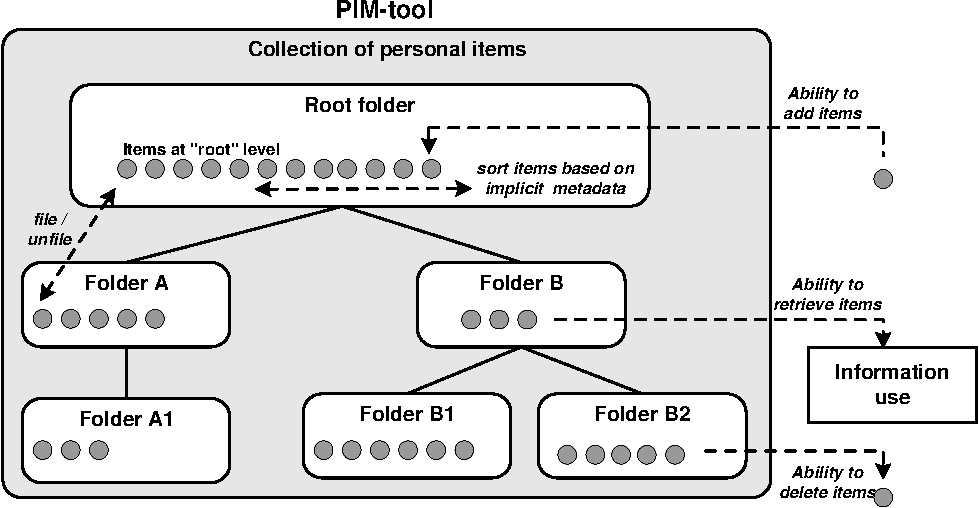
\includegraphics[height=6cm]{pictures/bg/BG-AbstractPimToolWithHierarchy.pdf}
		\caption{Model of a hierarchy-based PIM-tool}
		\label{fig:abstract_pim_tool_with_hierarchy}
	\end{center}
\end{figure}
%% Each item must also possess an index or label via which it can be accessed. Indices may be based on an explicit name (e.g. a filename) or implicit metadata (e.g. the subject line of an email).

\begin{itemize} % The user is enabled to manage items within an unfiled list at the ``top-level'', and within a hierarchy of folders.
\item \textit{Acquisition} -- items may be added as unfiled items in the top-level ``root'' folder, or placed directly into a low-level folder. 
%% ITEMS Can have implicit or explicit metadata. There may also be the potential to assign explicit metadata (e.g. name) to items.
%% items: minimum organizational unit

\item \textit{Organization} -- Explicit organization is enabled through the placement of items within folders. The user may change the folder structure by adding new folders, or renaming, deleting or moving existing folders.
% Implicit organization is carried out by the automatic assignment of implicit metadata such as size and date-created.
Typically, items are limited to placement in one folder location.  However, some folder hierarchy implementations allow the user to set-up \textit{links} or \textit{short-cuts} which can act as references from multiple locations to a particular item.

\item \textit{Maintenance} -- Typically, PIM-tools provide a mechanism to delete items. Implicit or explicit means of archiving may also be provided.

\item \textit{Retrieval} -- PIM-tools typically provide the ability to retrieve items from the collection through a combination of mechanisms. Firstly, users may browse through the hierarchy to retrieve items.  Two types of browsing can be highlighted: (1) browsing of folders, using user-defined explicit ``location'' metadata encoded in the folder structure; and (2) sorting/scanning of items within a folder, ordered by user-defined metadata (e.g. ``name'') or implicit metadata (e.g. ``date created''). The PIM-tool may also offer a search facility. Retrieved items may be re-saved within the hierarchy after editing.
% a sorting mechanism allows the user to order items in terms of their implicit metadata (e.g. date-created) or explicit metadata (e.g. name).  add types of browsing from CHI paper

\end{itemize}

Two types of interface are commonly employed to manage hierarchies: (1) a direct-manipulation file manager (pioneered in the Xerox Alto Neptune file manager~\citep{wadlow:81}), and (2) the command-line tools of UNIX or DOS. 

\textbf{Section~\ref{review:pim-theory-review}} surveys theory relating to PIM, including arguments in favour and against the use of hierarchical organization.



%%%%%%%%%%%%%%%%%%%%%%%%%%%
%%%%%%%%%%%%%%%%%%%%%%%%%%%
%%%%%%%%%%%%%%%%%%%%%%%%%%%
%%%%%%%%%%%%%%%%%%%%%%%%%%%

%%%%%%%%%%%%%%%%%%%%%%%%%%%%%%%%%%%%%%%%%%%%%%%%%%%%%%
\subsubsection{The Personal Information Environment}
\label{bg:pie}
%%%%%%%%%%%%%%%%%%%%%%%%%%%%%%%%%%%%%%%%%%%%%%%%%%%%%%
%% AKA workspace, activity space (Kirsh)

%%%%%%%%%%%%%%%%%%%%%%%%%%%
% PIE = physical + digital
%%%%%%%%%%%%%%%%%%%%%%%%%%%
The \textit{personal information environment} is defined as the aggregate of all collections of personal information. \textbf{Figure~\ref{fig:chapter2_pie}} offers a graphical summary of a personal information environment encompassing both the physical and digital domains.
%%%%%%%%%%%%%%%%%%%%%%%%
% FOCUS: digital PIE
%%%%%%%%%%%%%%%%%%%%%%%%
Note that the rest of this thesis focuses on the digital personal information environment which consists of:
% of all PIM-tools that allow an individual to manage personal information.  The personal information environment consists of the various interactive devices that allow an individual to manage personal information. These devices include:

\begin{enumerate}

\item \textit{Personal information collections stored on computers that the user has physical access to} -- Examples include desktop and laptop computers in work and home contexts.

\item \textit{Personal information collections stored on remote computers} -- As well as storing information on their local computer, the user may store information remotely on network drives.  Furthermore, many internet websites are now providing PIM-tool technology. Examples include web-based PIM-tools include email services (e.g. MS-Hotmail), on-line document management services, on-line calendars (e.g. Yahoo Calendar!), and shopping ``wish-lists'' stored on e-commerce sites such as amazon.com.

% In recent years, mobile devices such as cellular telephones and personal digital assistants have become commonplace. In addition it is common for people to own multiple computers at work and home. Due to this variety of digital devices people now manage personal information on multiple devices.
% A third trend is that of websites providing PIM-tool functionality. On one hand, many websites provide traditional PIM-tool-like functionality such management of email or to do-items. Also many e-commerce sites and on-line applications allow the user to manage collections of personal information relating to the site content. One example of this type is the amazon.com website which allows the user to manage a ``wish list'' of books they wish to purchase.

\item \textit{Personal information collections stored on mobile devices} -- Devices such as mobile phones and personal digital assistants (PDAs) are commonly used to manage contacts and notes.

% \item Personal information in the form of recorded messages stored in voice-mail systems

\end{enumerate}



% %%%%%%%%%%%%%%%%%%%%%%%%%%%%%%%%%%%%%%%%
% FIGURE - The Personal Information Environment
% %%%%%%%%%%%%%%%%%%%%%%%%%%%%%%%%%%%%%%%%
\begin{figure}[hbtp]
	\begin{center}
		\leavevmode
		%% [height=2in, width=.9\textwidth] 
		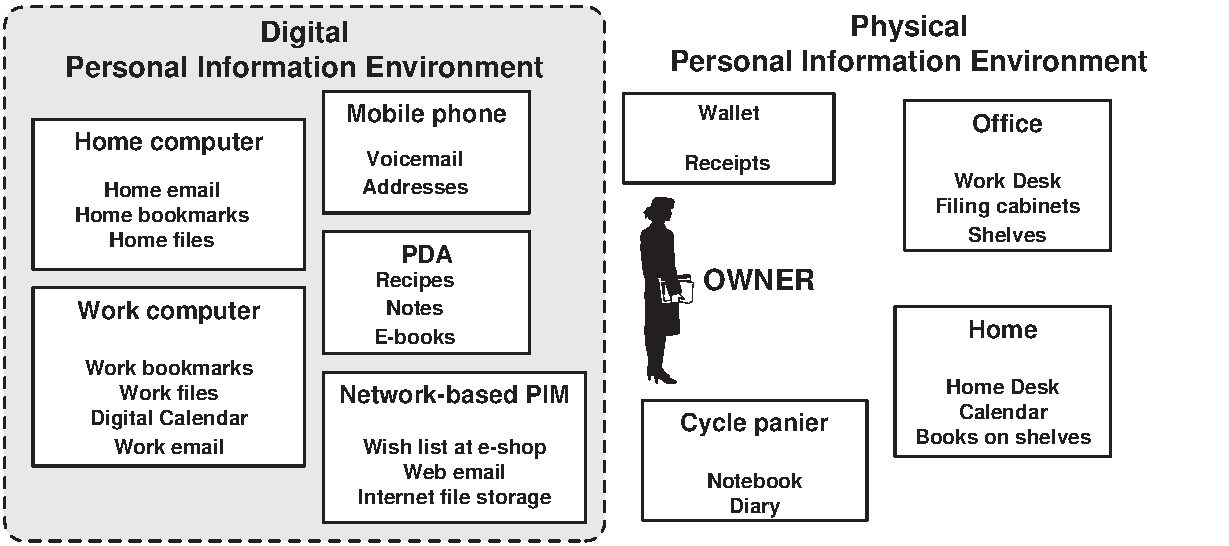
\includegraphics[width=.9\textwidth] {pictures/bg/BG-ExtendedPersonalWorkspace.pdf}
	\end{center}
	\caption{The personal information environment in both the physical and digital domains}
	\label{fig:chapter2_pie}
\end{figure}

%%%%%%%%%%%%%%%%%%%%%%%%%%%
%%%%%%%%%%%%%%%%%%%%%%%%%%%
%%%%%%%%%%%%%%%%%%%%%%%%%%%
%%%%%%%%%%%%%%%%%%%%%%%%%%%

\newpage
%%%%%%%%%%%%%%%%%%%%%%%%%%%%%%%%%%%%%%%%
\subsection{Trends in PIM-tool Design and Usage}
\label{bg:trends}
%%%%%%%%%%%%%%%%%%%%%%%%%%%%%%%%%%%%%%%%


Several ongoing trends can be identified in the design of PIM-tool technology:
\begin{enumerate}

% MORE USERS
\item \textit{Increasing numbers of users} -- With the boom in personal computing over the past decade,  millions of users now manage collections of email, files and bookmarks. Whereas in the past computer users were technically trained, today's PIM-tool users are from all walks of life and levels of technical expertise.  In other words, PIM tool technology is now a mass-market.

\item \textit{More collections of personal information} -- As noted in the previous section, today's personal information environment has evolved in a piecemeal incremental manner as new devices, PIM-tools, and technological formats have been invented.  This growth continues as more devices and websites offer PIM-tool functionality. 

%% trend/tension - bloating of tools (talk about in terms of task-artifact cycle)
%% ME: physical analogy - everyone has same desk and can paint/arrange different way. general-purpose, not designed with a specific user in mind
\item \textit{Increasing PIM-tool complexity} -- This increase in tool complexity is due to the addition of extra functionality and has been termed \textit{bloating}~\citep{mcgrenere:02}.  One reason for this phenomenon is that PIM-tools must cater for many possible approaches to managing personal information. PIM-tool developers must cater for all possible user groups -- from corporate users who depend on email during their working day, through to novice home users who may only check their email once a week. One example of the emerging complexity is that many email tools now provide integrated to-do item support. 
% A physical analogy might be millions of people sharing the same design of desk or diary. This genericity has contributed to the apparent trend towards increasing complexity in PIM-tools. 

\end{enumerate}

% These three trends -- increasing numbers of technically unsophisticated users, more collections of personal information, and   of more less technically sophisticated users, more collections and more complexity is problematic. % DISCUSS. 

%%%%%%%%%%%%%%%%%%%%%%%%%%%%%%%%%%%%%%
%% WHERE TO PLACE RESEARCH TRENDS??
%%%%%%%%%%%%%%%%%%%%%%%%%%%%%%%%%%%%%%
%% 2d/3d, speech-based systems
%% Such as 		\item Trend: increased intelligence/automation -- automation/overhead trade-off, limits of intelligent interfaces
%% 		\item Trend: Move away from the hierarchy? (see research prototypes below for more detail)
%% Move for/away from application.  No really a trend, more of a trade-off.  increasing specialization -- Tool-centric, embedding strategy/specialization strategy - Apple iApps

% \textbf{Section~\ref{bg:pie}} presents discusses the personal information environment, formed by the set of PIM-tools.
% discusses the trend towards the availability of more PIM-tools supporting the management of more types of personal information.
%% Then the trend towards increased integration is discussed in more detail in \textbf{Section~\ref{bg:integration}}.

%%%%%%%%%%%%%%%%%%%%%%%%%%%
%%%%%%%%%%%%%%%%%%%%%%%%%%%
%%%%%%%%%%%%%%%%%%%%%%%%%%%
%%%%%%%%%%%%%%%%%%%%%%%%%%%


%%%%%%%%%%%%%%%%%%%%%%%%%%%%%%%%%%%%%%%%%%%%%
\subsection{Integration between PIM-tools}
\label{bg:integration}
%%%%%%%%%%%%%%%%%%%%%%%%%%%%%%%%%%%%%%%%%%%%%
%% *********************
%% ADD: why integrate???
%% *********************
%% Application integration vs. data integration
%% hypertext-based integration
%% Mentions by Bellotti and Kaptelinin
%% Need to talk about the term `integration'?
%% Can we think about integration in terms of:
%		a) PIM tools / technological formats / collections
%		b) production activities
%		c) PIM sub-activities?
\textbf{Section~\ref{bg:pie}} described the historic trend towards multiple PIM-tools on multiple devices to form an extended personal information environment.  The provision of integration between PIM-tools is a key theme in this thesis.  This section offers a definition of integration, and surveys common integration mechanisms.
% This has lead to the need to provide integration between distinct PIM-tools.  

Although the term integration appears commonly in the marketing of PIM-tool software and other interfaces, there is no agreed definition in the research community.  The Oxford English Dictionary defines \textit{integration} as \textit{``the act or process of making whole or entire''}.  Here an integration mechanism is defined as a software component which provides user functionality that bridges two or more distinct PIM-tools.

\textbf{Figure~\ref{fig:chapter2_pim-tool_integration}} summarizes the integration mechanisms on a typical desktop computer running MS-Windows.  They are discussed as follows: % A survey of a typical Microsoft Windows machine reveals the following existing forms of integration between PIM-tools:
%% 
%% The terms integration and cross-tool defined, and current cross-tool mechanisms for integrating PIM tools are discussed.

\begin{enumerate}

\item \textit{Mechanisms that allows the user to initiate an operation in another PIM-tool} --  For example, right-clicking on an email address in an email message in MS-Outlook, allows the user to perform a search for that email address in the contact manager.
% to be taken to the address book (collection of contacts)
	
\item \textit{Mechanisms that allow information within one PIM-tool to be transferred to another PIM-tool} -- A simple example of this type is the ``cut-and-paste'' function provided by MS-Windows, e.g. copying some text from a file to an email.  Other ``higher-level'' operations combine the transfer of information with the initiation of an operation in the other PIM-tool., e.g. the ``Send-to'' mechanism allows a file to be attached within a newly created email message.
 %% send-to (example of add-on, bolt-on) (data transfer)

\item \textit{Mechanisms that allow items of various technological formats to be managed in a particular collection as ``primary-level items''} -- For example, MS-Windows allows the user to save email messages as a file within the file system. % An email saved in the file system is then equivalent to any other file.

\item \textit{Mechanisms that allow an items of various technological formats to be embedded within items of another format} -- Such embedded items are managed indirectly, via the item in which they are embedded.  An example of this type is email attachments: the ability to attach a file or bookmark within an email message. Typically, a reverse mechanism is also provided to allow the transfer of an attached item back to its native PIM-tool. % Clicking on an embedded item typically allows it to be opened within the foreign tool.

\item \textit{Retrieval mechanisms that bridge multiple tools} -- One example are cross-tool search mechanisms, e.g. SixDegrees~\citep{SixDegrees}, which allow the user to search multiple collections of information (e.g. files and email) in one operation. Some PIM-tools also permit cross-tool retrieval through browsing multiple collections. For instance MS-Windows Explorer allows the user to browse both the personal file system and the bookmark collection\footnote{The bookmark collection is stored within a special region of the MS-Windows file system in the ``Favorites'' folder.}.

\item \textit{Application suites that aggregate multiple PIM-tools} -- An example of this type is MS-Outlook which includes the PIM-tool functionality to manage five distinct collections of information: email, to-do items, notes, calendar and diary.

	% \item A final form of integration can be considered at the interface level in terms of consistency. Multiple PIM-tools often provide similar functionality such as search which are accessed via similar interfaces.
	
\end{enumerate}

% %%%%%%%%%%%%%%%%%%%%%%%%%%%%%%%%%%%%%%%%
% FIGURE - Integration between PIM-tools
% %%%%%%%%%%%%%%%%%%%%%%%%%%%%%%%%%%%%%%%%
\begin{figure}[hbtp]
	\begin{center}
		\leavevmode
		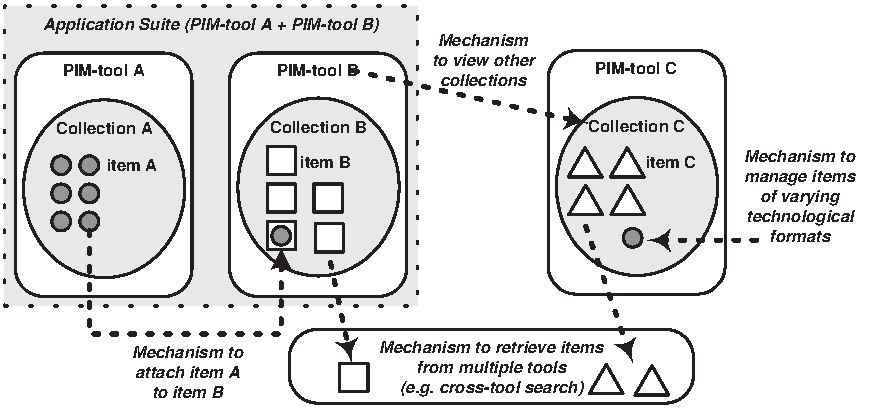
\includegraphics[height=6cm]{pictures/bg/BG-ToolIntegration.pdf}
	\end{center}
	\caption{PIM-tool integration mechanisms found in modern desktop operating systems}
	\label{fig:chapter2_pim-tool_integration}
\end{figure}

%% OTHER:
%% 
%% traversal between collections
%% All software applications are "integrated", can co-exist within the desktop graphical environment.

% It should be noted that all of these common integration approaches are effectively ``bolt-on'' mechanisms.
The range of integration mechanisms listed above is typical of most commonly available operating systems at the time of writing.  It should be noted that all of these common integration approaches are effectively ``bolt-on'' mechanisms.  Despite this wide range of integration mechanisms, information in different technological formats is managed in distinct collections within distinct PIM-tools.  

% CONTARST WITH SYNCHRONIZATION. \textit{Synchronization mechanisms that replicate items between collections of a particular technological format}. For example mirroring a work file system with one at home.  Not integration as the same technological format.

Note that this section has focused on integration available to ordinary users. Research aimed at improving integration is discussed in \textbf{Section 3.5}, including systems that unify the management of multiple types of information within a consolidated interface.
%% TODO: update section number!!
%% Simple context-aware: Nardi and co. - Data Detectors (example of research that became part of a commercial product)~\cite{bn:98}



%%%%%%%%%%%%%%%%%%%%%%%%%%%
%%%%%%%%%%%%%%%%%%%%%%%%%%%
%%%%%%%%%%%%%%%%%%%%%%%%%%%
%%%%%%%%%%%%%%%%%%%%%%%%%%%

%%%%%%%%%%%%%%%%%%%%%%%%%%%%%%%%%%
%\subsection{Summary}
%\label{bg:summary}
%%%%%%%%%%%%%%%%%%%%%%%%%%%%%%%%%%

% \textbf{Section~\ref{bg:pim-tools}} provided further conceptual background to the thesis by introducing PIM-tools. Personal computer users have access to a powerful existing set of PIM-tools allowing them to manage a range of types of information. Studies of tool usage are described in \textbf{Chapter~\ref{chapter:review}}.
%%
%% Relate to reported user problems: link towards HCI studies to follow.  Need for more design work? Users have powerful set of tools.  What is missing?

%%%%%%%%%%%%%%%%%%%%%%%%%%%
%%%%%%%%%%%%%%%%%%%%%%%%%%%
%%%%%%%%%%%%%%%%%%%%%%%%%%%
%%%%%%%%%%%%%%%%%%%%%%%%%%%

%% \newpage
%%%%%%%%%%%%%%%%%%%%%%%%%%%%%%%%%%
%%%%%%%%%%%%%%%%%%%%%%%%%%%%%%%%%%
\section{Summary}
\label{bg:conclusion}
%%%%%%%%%%%%%%%%%%%%%%%%%%%%%%%%%%
%%%%%%%%%%%%%%%%%%%%%%%%%%%%%%%%%%

% This section presents the main conclusions of \textbf{Chapter 2}.
\textbf{Section~\ref{bg:pim}} offered a conceptual framework detailing the view of PIM taken in this thesis, as  an activity consisting of four sub-activities: acquisition, organization, maintenance, and retrieval. \textbf{Section~\ref{bg:pim-tools}} defined a PIM-tool as a software component which enables the user to manage a collection of personal information. A survey of existing PIM-tool technology was also provided, along with a discussion of their evolution from early multi-user systems.
%%
%% that define key concepts and terms for discussing (1) PIM as an activity, and (2) the tools that facilitate PIM.

\textbf{Chapter~\ref{chapter:review}} moves on to review relevant research carried out within Human-Computer Interaction and other related disciplines, aimed at investigating user needs regarding PIM, and designing improved technology to support it.

%%%%%%%%%%%%%%%%%%%%%%%%%%%%%%%%%%%%%%%%%%
%% Mention relationship to other chapters:
%%%%%%%%%%%%%%%%%%%%%%%%%%%%%%%%%%%%%%%%%%
%% 
%% PIM conceptual framework developed in more depth in Chapter 4?
%% Reiterate PIM as an appication domain within HCI.
%% Now move onto next chapter: a review of previous research on PIM within HCI and related disciplines. 

%%%%%%%%%%%%%%%%%%%%%%%%%%%%%%%%%
% FIN THESIS CHAPTER 2: BACKGROUND
%%%%%%%%%%%%%%%%%%%%%%%%%%%%%%%%%
% \textit{This draft of ``Chapter 2 Background'' was printed \today}
